% !TEX root = ../main.tex

\chapter{Machine Learning}
We apply PNN(Probabilistic Neural Network) for machine learning.PNN can be regarded as a Radial Basis Neutral Network,it’s based on the Radial Basis Function(RBF) network and involved Density function estimation and Bayesian decision theory.Under most conditions,PNN can realize the discriminant boundary asymptotically approaching the Bayesian optimal decision surface.
\section{Neural network structure of PNN}
PNN is consist of input layer,Radial Basis Layer(hidden layer) and competitive layer(output layer),which is shown in ~\ref{fig:structure of PNN}.The first layer is the input layer,it’s used to receive training sample and transfer data to hidden layer.The hidden layer is Radial basis layer,it receives samples form the input layer and return a scalar which depends on the Euclidean distance to the center vector.the scalars are transferred to the output layer,which is a competition layer,which can output the scalar that satisfy the competition requirement.During the training process,we are able to achieve the center vector and variance of each class.In the later testing process,through calculating the Euclidean distance from the sample to each center vector and transform into the probability of decision based on Bayesian optimal decision.
\begin{figure}
    \centering
    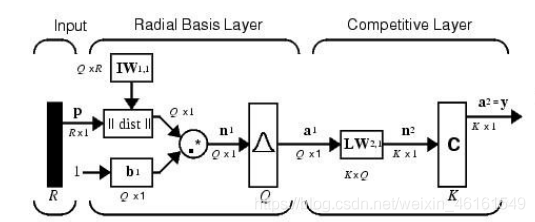
\includegraphics[width=0.9\textwidth]{figures/PNN neural network.png}
    \caption{structure of PNN}
    \label{fig:structure of PNN}
\end{figure}
\subsection{Radial Basis Function(RBF)}
The main idea of the RBF layer is using the RBF as the basis of the latent space,this allows the input vector to be directly mapped to the latent space without connecting through weights.When the center point of the RBF is determined after the training process,the mapping relationship is also determined.Among them, the role of the hidden layer is to map the vector from the low-dimensional \verb+p+ to the high-dimensional \verb+h+, so that the low-dimensional linear inseparability can become linearly separable to the high-dimensional,which is the main idea of the kernel function. In this way, the mapping of the network from input to output is nonlinear, while the network output is linear with respect to adjustable parameters. The weights of the network can be directly solved by the linear equation system, which greatly speeds up the learning speed and avoids the local minimal problem.
the activative function of the raidal basis neural network can be written as
\begin{equation}
\operatorname\\{R}({x}_{p}-{c}_{i})=
\\exp{(-\frac{1}{2\,\sigma_i^2} \Vert {x}_{p}-{c}_{i}\Vert_2^2})
\end{equation}
As we can see,if the sample vector ${x}_{p}$ is closed to the center vector ${c}_{i}$,$R$ would be more closed to $1$,based on this,we are able to build the connction from $R$ to the probability of decision through Bayesian optimal decision.
\subsection{Bayesian optimal decision theory}
The competition layer(output layer)is based on the Bayesian optimal decision theory.
for a typicalbinary classification problem: $c=c_1$ or $c=c_2$.Prior probability can be written as
\begin{equation}
{h}_{1}=\\{p}({c}_{1}),{h}_{2}=\\{p}({c}_{2}),{h}_{1}+{h}_{2}=1
\end{equation}
for any input vector $x = [x_1,\ldots,x_n]$,the classification criterion are shown below:
\begin{equation}
    {c}=
    \begin{cases}
    c_1,p(c_1|x)>p(c_2|{x}),\\
    c_2,otherwise
    \end{cases}
\end{equation}
${p}({c}_{i}|{x})$ is defined as when $x$ happens,the posterior probability of $c_i$.According to the Bayesian function.the posterior probability equals to 
\begin{equation}
    p(c_i|x)=\frac{ p(c_i)p(x|c_i)}{ p(x)}
\end{equation}
during the decision making process,the classification criterion should be the posterior probability.In practical situation,cost of misclassification are need to be considered.The cost of missclassify type 1 sample into type 2 and missclassify type2 sample into type1 are sometimes different.Therefore,the classification are needed to be adujusted.Define event $\alpha_{1}$ is classify the input vector into type $c_i$,the cost of misclassification is $\lambda_{ij}$.So the expectation cost of apply event $\alpha_{1}$ is
\begin{equation}
    \\R(\alpha_i|\\x)=\sum_{j=1}^{N} \lambda_{ij}\\p(c_i|\\x)
\end{equation}
Assume that the cost of correctly classification is $0$,the expectation cost of event $\alpha_{1}$ is
\begin{equation}
     \\R(\alpha_i|\\x)= \lambda_{12}\\p(c_2|\\x)
\end{equation}
The Bayesian theorem turns into
\begin{equation}
    {c}=
    \begin{cases}
    c_1,R(c_1|x)<R(c_2|{x}),\\
    c_2,otherwise
    \end{cases}
\end{equation}
However,in the project,we assume that the cost of missclassification are equals,so the classification only depends on the probability of events.
\section{Summary of implementing PNN}
Firstly,based on the label of the training set,we are able to attain the center vector $u_j$ and variance $\sigma_j$ of class $j$.
\begin{equation}
    u_j=min{\sum_i}\Vert x_{ij}-u_j\Vert_2^2\\
\end{equation}
\begin{equation}
    \sigma_j=\sqrt{\frac{1}{N}\sum_{i=1}^{N}\Vert x_{ij}-u_j\Vert_2^2}
\end{equation}
where $K$ is the number of class $j$.
\par
Secondly,for each new sample $x_i$ in the testing layer,we apply the RBF to transform the Euclidean distance between $x_i$ and center vector of each classes $u_j$ into a real number $\phi_{ij}$ ranging from $0$ to $1$.then,we normalize $\phi_{ij}$ and regard it as the probability of classification.
\begin{equation}
    \phi_{ij}=\\exp{(-\frac{1}{2\,\sigma_j^2} \Vert {x}_{ij}-{u}_{j}\Vert_2^2})
\end{equation}
\begin{equation}
    p_{ij}=\frac{\phi_{ij}}{\sum_{j}\phi_{ij}}
\end{equation}
which means the probability of classifying sample $x_i$ into class $j$.
\par
Lately,we apply the Bayesian optimal theorem as the decision criterion and output the result.
\par
In order to clearify and simplify the result,we only select several singer's songs as the entire sample.randomly choose $80\%$ of the entire sample(16891) as the training set while the rest $20\%$(4222) is the testing set.the Accuracy of the training set and the testing set are around $97\%$(shown in \ref{fig:estimationresult}),which indicates the effectiveness and accuracy of the PNN to the problem.
\begin{figure}[b]
    \centering
    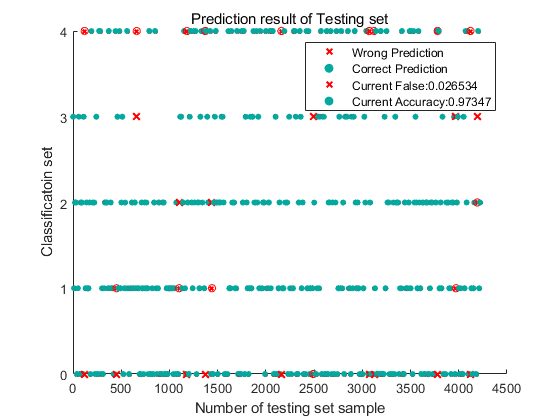
\includegraphics[width=0.85\textwidth]{figures/zxt/estimationresult.png}
    \caption{Prediction result of Testing Set}
    \label{fig:estimationresult}
\end{figure}